


\Aufgabe{Gameboard-Library}

\doppelseite{0.47}{0.47}{t}
{%
Die Gameboard Library stellt im package \emph{bbe} ein fertiges \emph{Gameboard} zur Verfügung, zu dem Objekte (so genannte Entities) hinzugefügt werden können. Zur Festlegung der Darstellung der Entities können (aber müssen nicht!) verschiedene Methoden implementiert werden, die rechts in der Klasse \emph{ExampleEntity} dargestellt werden.

Weitere Informationen zu den Methoden gibt es im Struktogramm auf der nächsten Seite und unter \href{https://gameboard.valentin-herrmann.com}{gameboard.valentin-herrmann.com}

\vspace{0.5cm}
\begin{tikzpicture}
\begin{class}[text width=\linewidth]{Gameboard}{0 ,0}

\operation{+ Gameboard()}
\operation{+ void add(Object obj)}
\operation{+ void remove(Object obj)}
\operation{+ void clear()}
\operation{+ void start(String title)}
\operation{+ void setBackgroundImagePath(String path)}
\operation{+ void setShowHitboxes(boolean show)}
\operation{+ Object[] getObjects()}

\end{class}
\end{tikzpicture}
}
{%
\begin{tikzpicture}
\begin{class}[text width=\linewidth]{ExampleEntity}{10 ,0}

\operation{+ Number getX()}
\operation{+ Number getY()}
\operation{+ String getText()}
\operation{+ String getImagePath()}
\operation{+ double getScaleFactor()}
\operation{+ boolean isStatic()}
\operation{+ String getGameoverMessage()}
\operation{}
\operation{+ void setLeft(boolean pressed)}
\operation{+ void setRight(boolean pressed)}
\operation{+ void setUp(boolean pressed)}
\operation{+ void setDown(boolean pressed)}
\operation{+ void setW(boolean pressed)}
\operation{+ void setA(boolean pressed)}
\operation{+ void setS(boolean pressed)}
\operation{+ void setD(boolean pressed)}
\operation{+ void setEnter(boolean pressed)}
\operation{+ void setSpace(boolean pressed)}
\operation{}
\operation{+ void crash()}
\operation{+ void crash(String className)}
\operation{+ void crash(Object other)}
\operation{+ void crash(String className, Object other)}


\end{class}
\end{tikzpicture}
}

\vspace{0.5cm}

\textbf{Gameboard in der Main-Methode erzeugen:}

\normalsize
\begin{verbatim}
import bbe.Gameboard;                     // Gameboard Library importieren
public static void main(String[] args) {  // Methodenkopf von main
   Spieler spieler1 = new Spieler();      // Spieler erstellen
   Gameboard spiefeld = new Gameboard();  // Gameboard erstellen
   spielfeld.add(spieler1);               // Spieler zum Gameboard hinzufügen
   spielfeld.start("Spiel");              // Spiel mit Fenstertitel "Spiel" starten
}
\end{verbatim}

\large
\textbf{Gameboard in BlueJ graphisch erzeugen:}

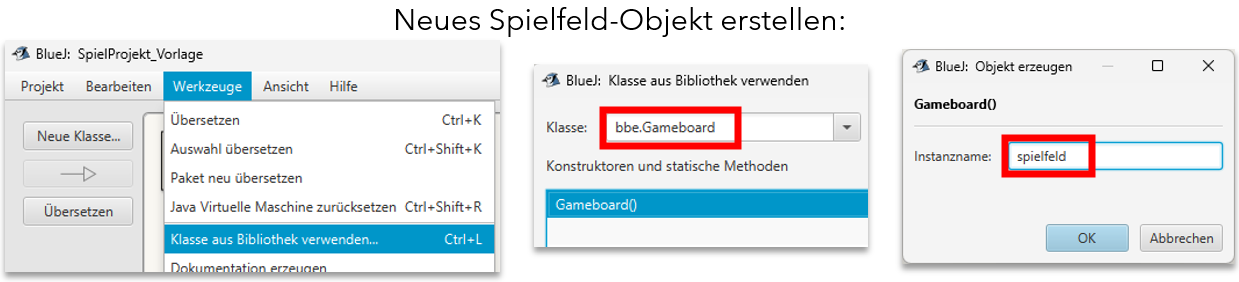
\includegraphics[width =\textwidth]{_Aufgaben/BlocklyJava_Skript/img/A10_CreateGB.png}



\begin{minipage}{\textwidth}
\subsection*{Interner Ablauf des Gameboards}

Dieses Struktogramm stellt den internen Ablauf des Gameboards beim Ausführen des Spiels dar. 

\fbox{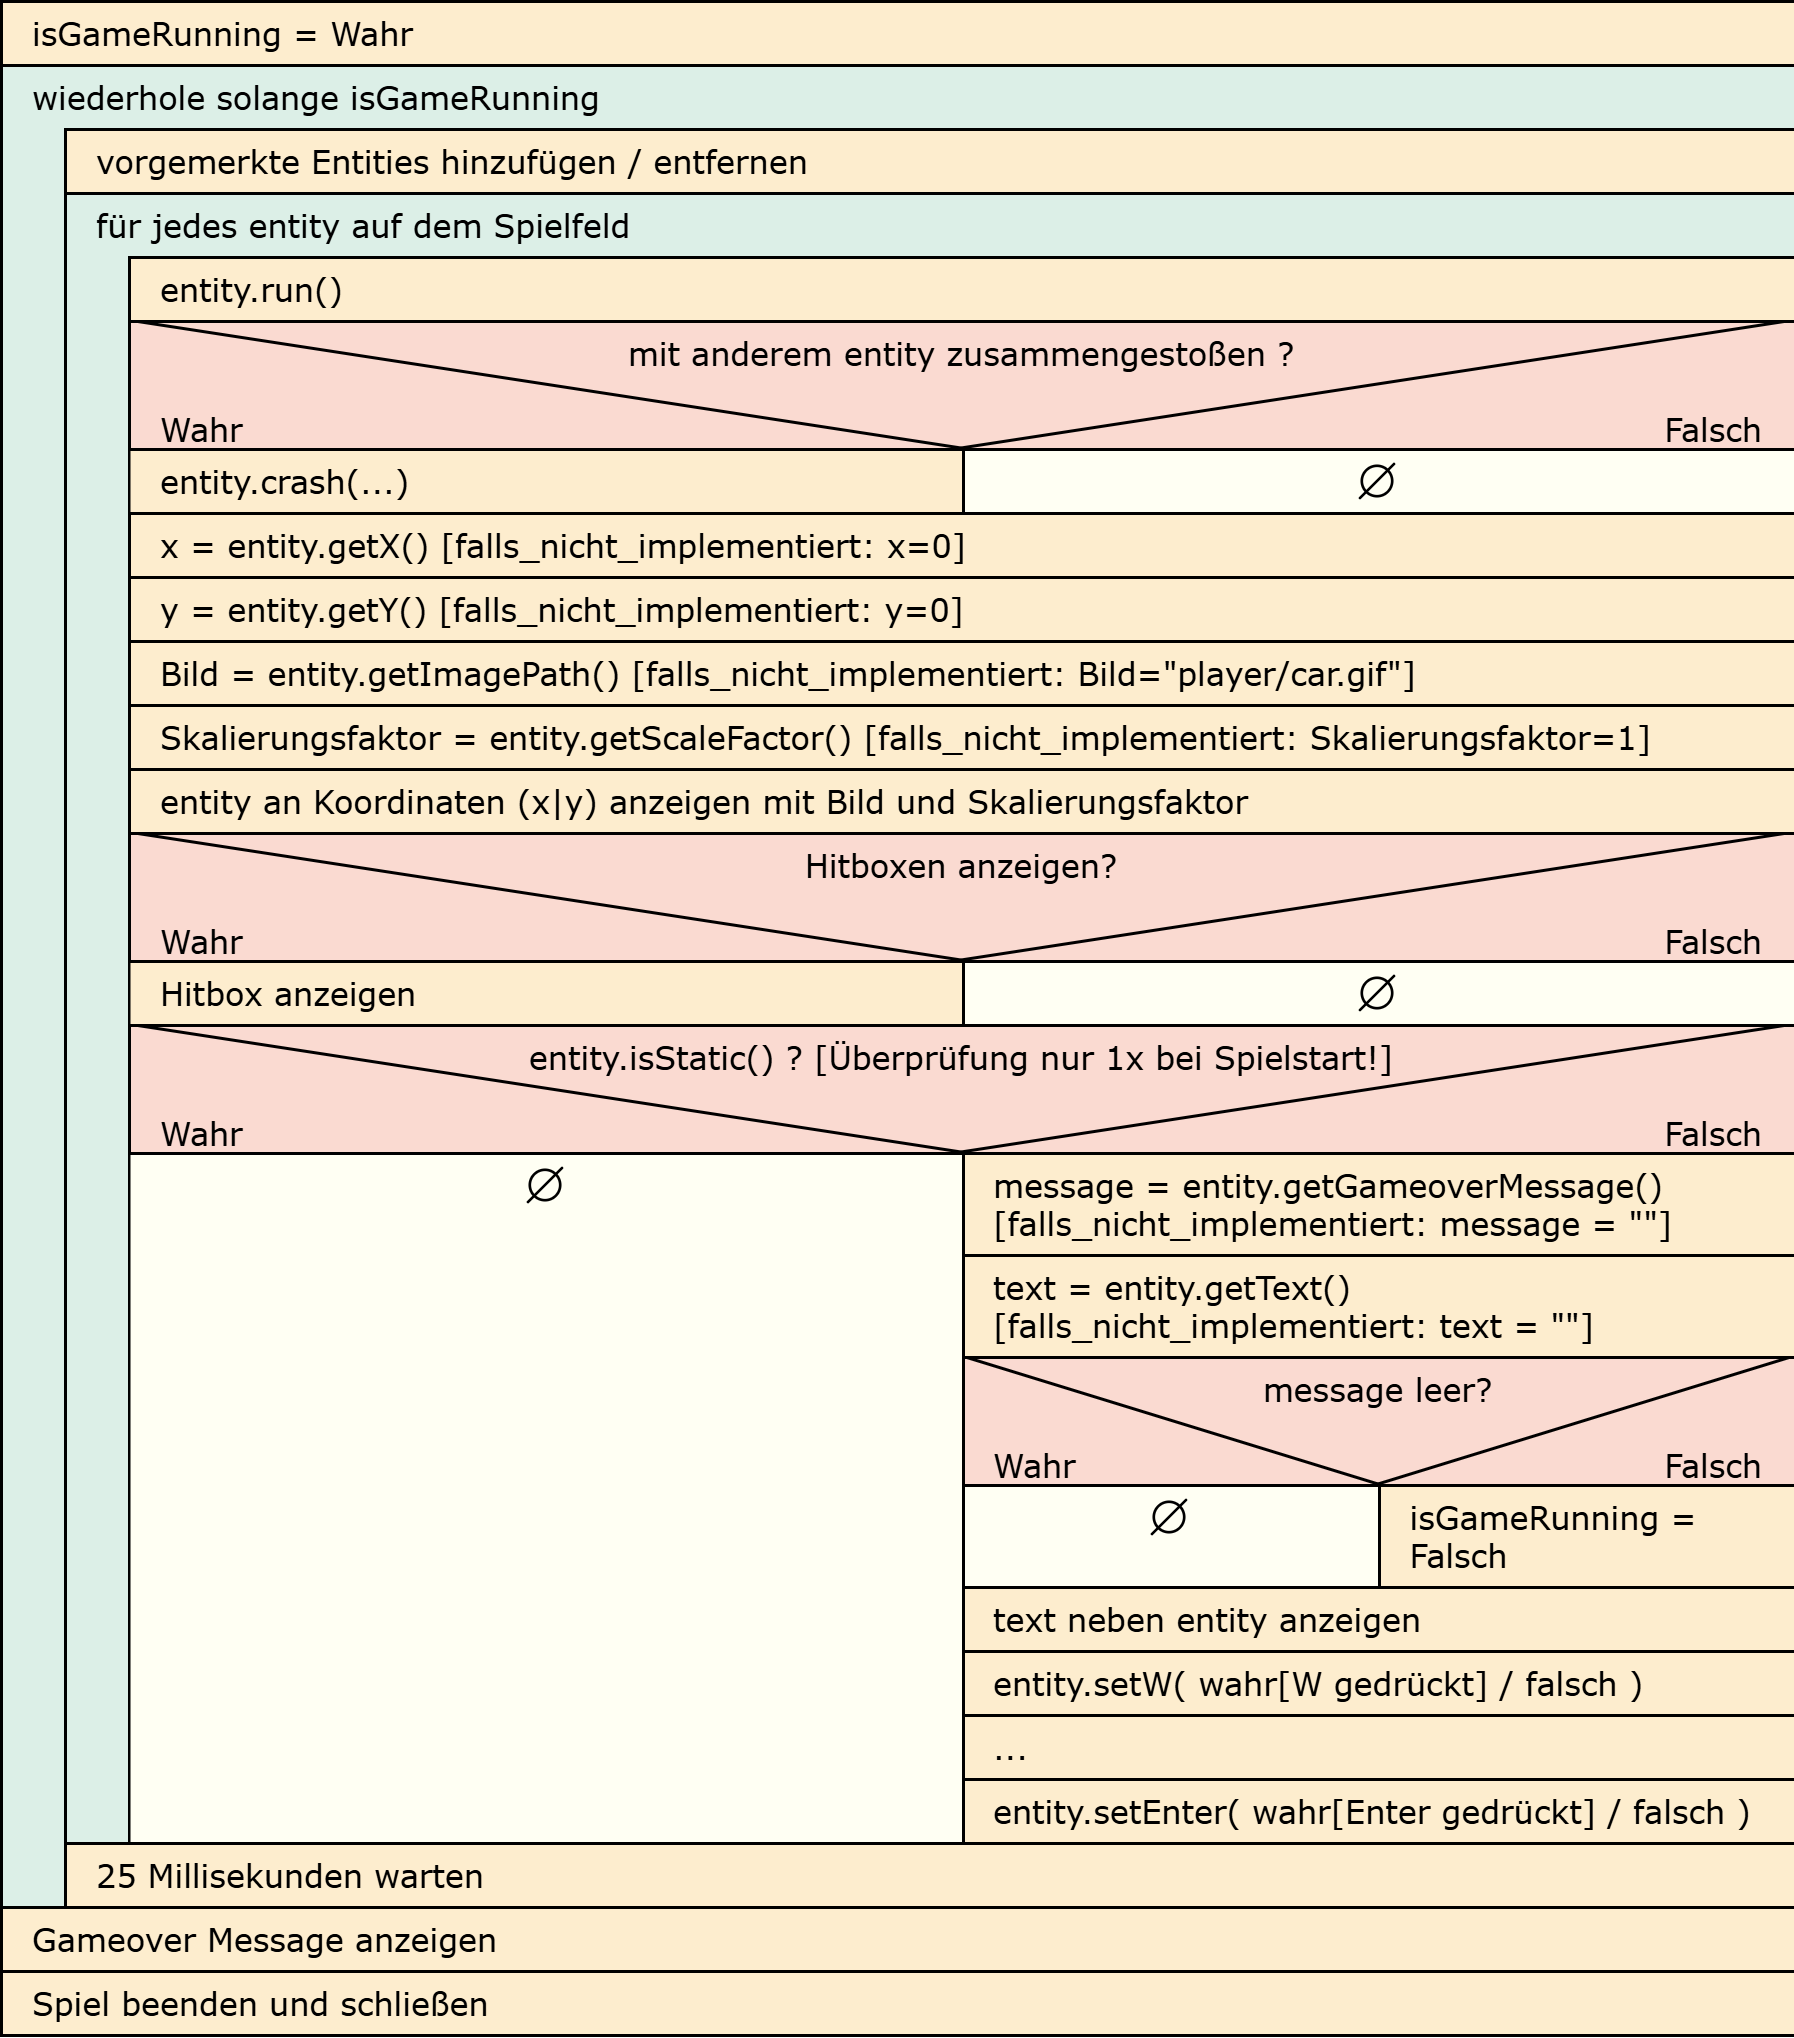
\includegraphics[width=\textwidth]{_Aufgaben/BlocklyJava_Skript/img/P_struktog_Gameboard.png}}
    
\end{minipage}